\section{Unit 3D} % (fold)
\label{sec:unit_3d}

A unidade é um ecossistema de desenvolvimento de jogos com ambiente integrado à: 

\begin{itemize}
	\item Motor de renderização
	\item Conjunto de ferramentas e fluxos de trabalho para criar 3D interativo e conteúdo 2D
\end{itemize}

Além de oferecer as simplicidades de:
\begin{itemize}
	\item Publicação multiplataforma,
	\item Template de asserts disponíveis em loja interna,
	\item Comunidade ativa,
\end{itemize}

O Unity é muito interessante para desenvolvedores e estúdios independentes por agiliza a produção de uma ambiente funcional a um custo muito baixo, podendo vir a ser gratuita a licença.

\subsection{Workflow} % (fold)
\label{sub:workflow}

	Com o intuito de simplificar o processo de criação e produção de software, o Unity oferece um ambiente de trabalho com diversas ferramentas integradas para o desenvolvimento, permitindo que em um mesmo ambiente possa ser feito ajustes de modelagens, acentuação de peças, produção de cenas e ate mesmo a implementação de scripts para o \textit{gameplay}.

\begin{figure}[h]
  \centering
  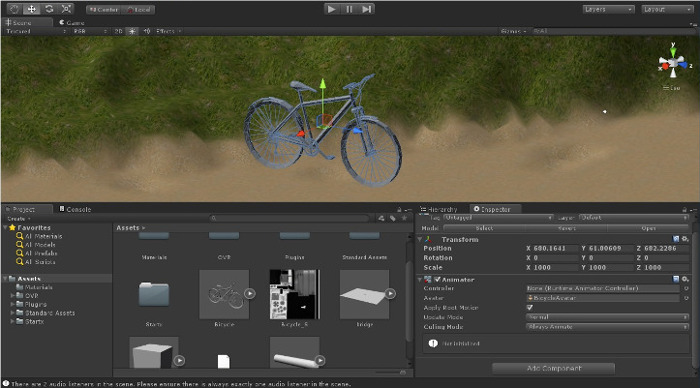
\includegraphics[width=0.8\textwidth]
      {figuras/bike.png}
  \caption{Edição de objeto no Unity}
  \label{coordenadas-rift}
\end{figure}

Apesar de permitir um trabalho de \textit{design} dentro do Unity, é possível importar um objeto modelado em ferramentas dedicadas para a modelagem de objetos, como o Maya\footnote{Mais informações em \url{www.autodesk.com.br/products/maya/overview}} ou o Blender\footnote{Mais informações em \url{www.blender.org}}, facilitando não apenas no \textit{design} do objeto, mas animações também.


\begin{figure}[h]
  \centering
  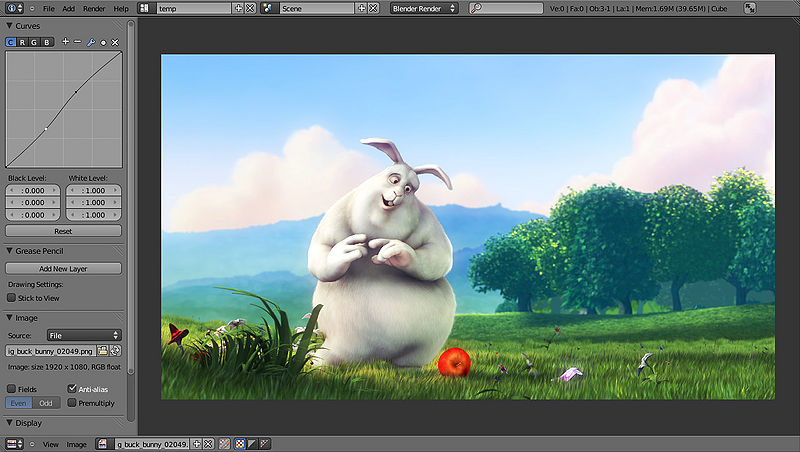
\includegraphics[width=0.8\textwidth]
      {figuras/blender.png}
  \caption{Renderização de \textit{Bick Buck Bunny} sendo feita no Blender}
  \label{coordenadas-rift}
\end{figure}

\subsection{Multiplataforma} % (fold)
\label{sub:multiplataforma}

Infelizmente, o ambiente de desenvolvimento do Unity não possuiu executável para Linux ainda, porém é capaz de gerar builds para diversas plataformas, incluindo Linux e consoles da atual geração, totalizando um total de 16 plataformas. 

O interessante é que a própria plataforma de desenvolvimento faz uma filtragem dos scripts e edição com a plataforma, permitindo que seja inseridos vários scripts no projeto, cada um dedicado à plataformas especificas.

Além disso, o Unity possuiu uma ferramenta -\textit{Unity Remote} -  que permite a depuração do código de forma remota na plataforma alvo.

